\documentclass[a4paper,12pt]{report}
\usepackage{graphicx}
\usepackage[T1]{fontenc}
\usepackage[utf8]{inputenc}
\usepackage{blindtext}
\usepackage[french]{babel}


\begin{document}
	\chapter{Cadre du projet :}
	\newpage
	
	
	\section{Introduction :}
	Ce chapitre est consacré à la présentation de cadre de projet. Il est subdivisé en  parties.
	la première partie est consacrée au problématique , la deuxième
	porte l'etude d'existant, la troisiéme détermine la  solution proposé, la quatreieme partie porte l’objectif, et la dernière spécifie la Méthodologie de gestion de projet.
	\section{Problématique :}
	Depuis des temps immémoriaux l'agriculture tunisienne était trés importante dans la meusure où elle faisait partie intégrante de la vie humaine.
	\par
	Néanmoins ce secteur central a étalé une faiblesse importante de compétivité sur les marchés nationaux et internationaux suite à un manque de la technique et de l'innovation qui reflète une faible production et l'absence de qualité des produits agricoles d'organisations professionnelles bien développée.
	
	\section{Etude de l’existant :}
	
	Donc on a besoin d'un système de détection couvrent les plantations, rangée par rangée, grâce à une quadri rotor. Les données recueillies par le système sont ensuite analysées et traitées à l’aide de l’Intellegence Artificielles, afin d’identifier les oranges de chaque arbre. Les résultats sont alors transmis au producteur et sont accessibles sur l'appareil.
	\section{Solution proposée: }
	Après avoir étudié attentivement ce sujet, l'observation et l'analyse des problèmes qui résultent de ce sujet . Nous avons bien conclu qu'il faut créé une progression au niveau de ce secteur, concevoir des solutions qui peuvent augmenter la qualité et la production de l'agriculture et aider les agriculteurs à avoir une progression au niveau de la compétitivité dans ce domaine-là . Dans ce contexte, nous avons mis en place un système innovant focalisé sur l'application d'un drone pour la détection des oranges .
	\par
	Ce système est divisé en deux parites :
	\par
	- drone 
	\par
	- détection des oranges
	\newpage
	\section{Objectif :}
	Quelle est l'objectif de l'agriculture ?
	Répondre aux besoins des populations. Garantir une production suffisante Réduire les écarts de richesse. Garantir l'équilibre du milieu naturel.  limitant la fatigue des opérateurs et l’impact
	Les systèmes d’agriculture intelligente et de précision devraient jouer un rôle important dans
	l’amélioration des activités agricoles.
	e plus productives, plus efficaces
	et plus rentables
	, cependant de telles technologies ne suffisent pas à elles seules; elles doivent être
	combinées judicieusement avec des outils puissants d’exploration de données pour fournir des informations pertinentes, utiles et fiables.
	Les drones sont en mesure de fournir des données de manière rapide et précise, ce qui permet de livrer les projets plus vite et facilite la prise de décision.
	
	
	
	Afin de s’organiser de manière appropriée, les agriculteurs ont besoin d’anticiper leur production. Mais le comptage des fruits est une tâche qui prend du temps. Le projet AGERPIX, soutenu par l’UE, a permis de mettre au point une méthode de travail plus efficace pour les fournisseurs de produits agricoles: un système automatisé de comptage des fruits sur l’arbre.Un système de comptage des fruits très précis utilise l’intelligence artificielle pour aider les producteurs à optimiser leurs récoltes et à planifier leurs ventes sur le marché.
	
	\section{Méthodologie de gestion de projet :}
	\subsection{Choix de méthodologie :}
	Afin d'assurer le bon déroulement des différentes étapes
	Dans notre projet, nous avons choisi la méthode Agile Scrum pour gérer notre travail, concevoir et
	Développer nos systèmes pour des raisons claires est vraiment le processus
	Scrum s'inscrit parfaitement dans la décomposition de notre projet de fin d'etudes, qui s'appuie sur des avantages suivants :
	\par
	Plus de flexibilité et de réactivité.
	\par
	traduire et organiser le projet de façon simple, transparente et pragmatique.
	
	\subsection{C'est quoi Scrum :}
	Scrum est la méthode agile la plus utilisée. A l'instar des autres méthodes agiles, Scrum est une démarche de gestion de projet qui fait du client (ou utilisateur) le principal pilote de l'équipe en charge des développements.
	\subsection{Présentation de la méthodologie scrum :}
	La méthode SCRUM implique que le projet progresse à travers la mise en place de séries de « sprints ». À chaque lancement d’un sprint, une réunion de planification est organisée afin que chaque membre de l’équipe puisse s’engager sur le nombre de tâches qu’il pourra exécuter, ainsi que sur la création du « sprint blacklog ».
	Chaque jour du sprint, tous les membres de l’équipe (ainsi que le responsable produit et le SCRUM Master) doivent assister à la réunion SCRUM quotidienne. Cette dernière ne doit pas durer plus de 15 minutes, et permet aux membres de l’équipe de partager avec les autres ce qu’ils ont fait la veille, ce sur quoi ils travaillent le jour même, ainsi que l’identification de tout problème pouvant entraver le bon déroulement du sprint. Cette réunion permet ainsi de synchroniser tous les membres de l’équipe.
	\par
	La fin d’un sprint est marquée par une session de débriefing permettant de présenter le travail achevé au responsable produit, et de partager des informations pouvant influer sur le sprint suivant.
	\begin{figure} [h]
		\begin{center}
			\centering
			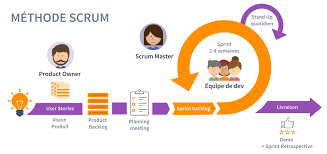
\includegraphics[width=1\linewidth]{Images/téléchargement (4)}
		\end{center}
		\caption{Méthode scrum}
	\end{figure}
	\subsubsection{product owner :}
	Personne ayant la responsabilité de produire et de maintenir à jour le carnet de produit. C'est lui qui détermine les priorités et qui prend les décisions d'orientation du projet .
	\subsubsection{scrum master  :}
	Membre de l'équipe dont l'objectif principal est de la protéger des perturbations extérieures. Il est complètement transparent pour la communication entre l'équipe et les clients et n'a aucun pouvoir hiérarchique sur l'équipe. C'est en revanche un facilitateur pour les problèmes non techniques de l'équipe .
	\subsubsection{product backlog  :}
	Liste des fonctionnalités, des fonctions, des exigences, des améliorations et des correctifs qui sont nécessaires à l'évolution du produit , celui-ci est dynamique sur tout le cycle de vie du produit.
	sprint backlog  :
	Liste des tâches à accomplir pendant un sprint. Elles correspondent à la réalisation des éléments de carnet de produit affectés au sprint .
	\subsubsection{sprint :}
	Nom d'une itération dans Scrum. Cette itération dure 1 mois maximum en théorie, mais en pratique entre 2 et 4 semaines. Pendant une itération, l'équipe doit développer la liste d'éléments du carnet de produit qui a été définie au début du sprint.
	\subsection{Outils destinés à la gestion du projet :}
	\subsubsection{Google Drive}
	Google drive est un outil de partage et de collaboration utilisé pour travailler sur les différents
	documents à produire au cours de la session. Tous les documents qui ne sont pas du code sont
	centralisés sur cette application
	\begin{figure} [h]w
		\begin{center}
			\centering
		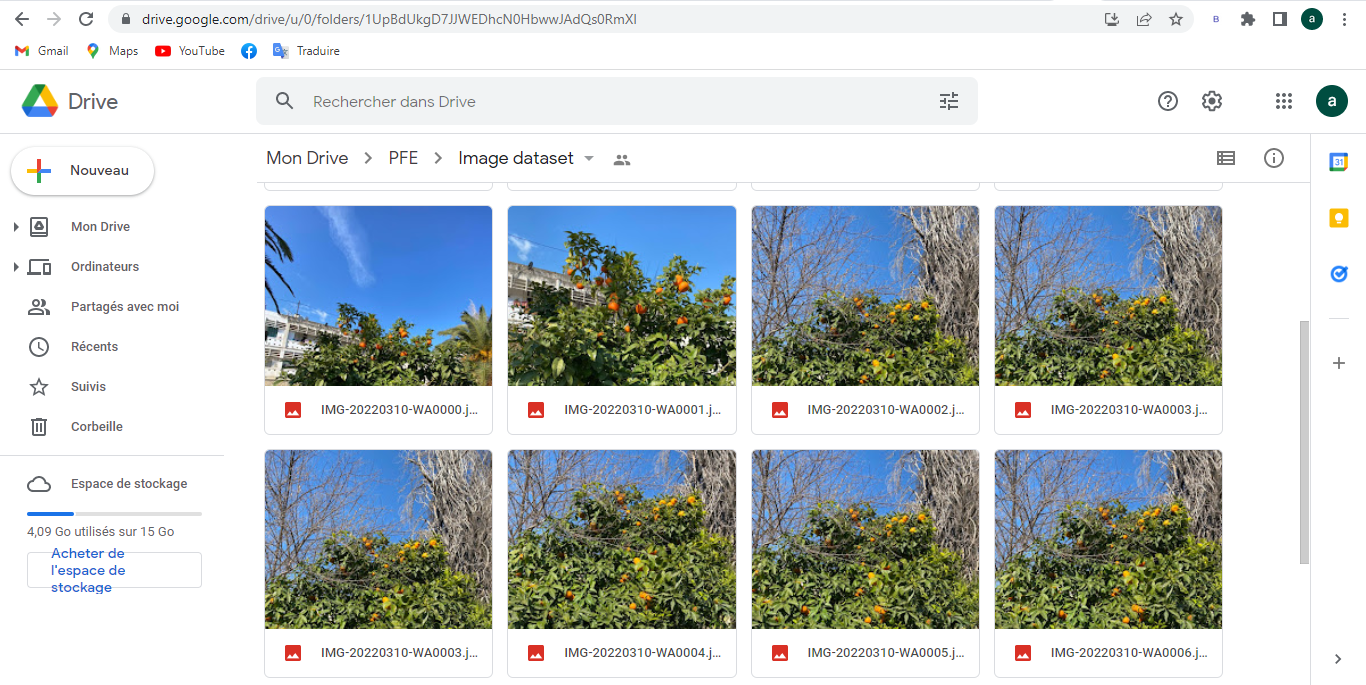
\includegraphics[width=0.7\linewidth]{Images/2022-04-09 (7)}
		\end{center}
		\caption{aaa}
	\end{figure}
	\newpage
	\subsubsection{Jira Software}
	La sélection de jira software comme étant un outil de gestion de notre projet puisque q'il est un outil puissant car on peut visualiser l'avancement de notre travail grâce aux tableaux Agile, effectuer un reporting de qualité à l’aide des tableaux de bord et travailler à distance grâce à cette platforme Jira software.
	Développé par l'entreprise australienne Atlassian, Jira Software, le produit phare de l'éditeur, est un logiciel principalement dédié à la gestion de projet de développement d'applications en mode agile.
	\subsubsection{Github}
	Github est utilisé pour la centralisation et la gestion du code source , des documets et des différents modules du projet. Ce service est utilisé puisque le projet se trouvait déjà sur cette plateforme et qu’elle est
	facile à utiliser.
	\begin{figure} [h]
		\begin{center}
			\centering
			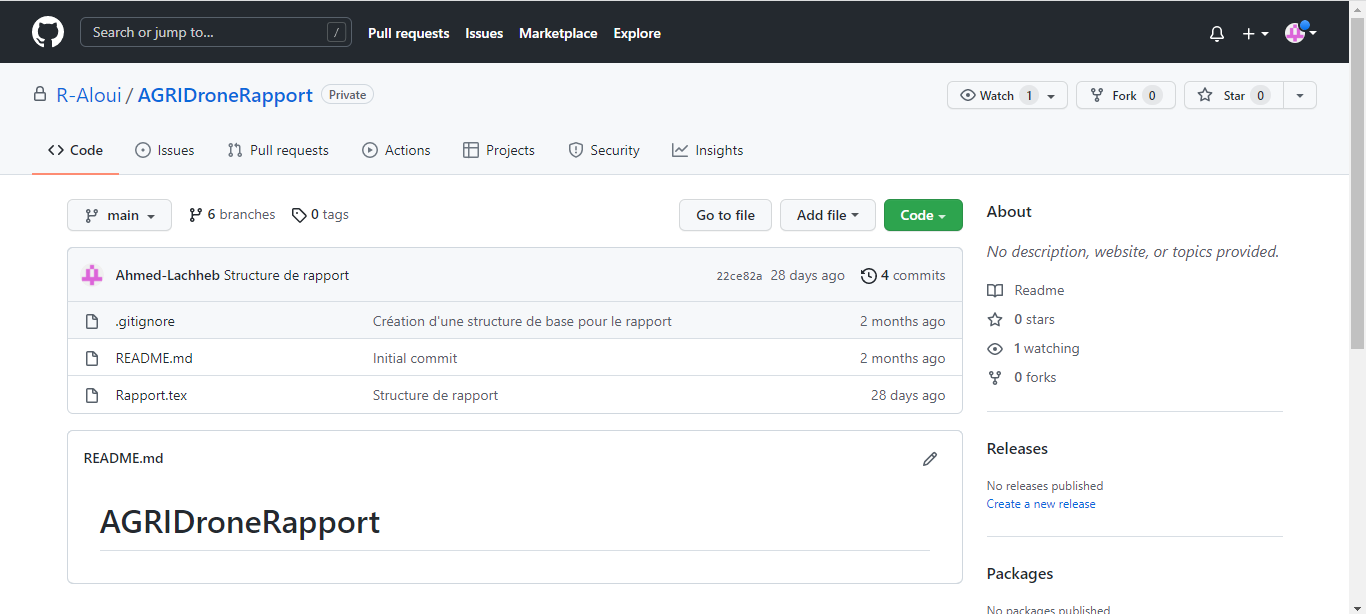
\includegraphics[width=0.7\linewidth]{Images/2022-04-09 (6)}
		\end{center}
		\caption{Méthode scrum}
	\end{figure}
\end{document}